\section{Address Translation}

After a device's configuration is determined, if the device is subject to address
translation, either one-stage or two-stage, The IOMMU performs the address translation
with another set of memory-resident table structure referred to as the \textit{Address
Tables}. During the translation, the IOMMU uses the virtual address and access type of the
memory access and output a physical address or raises a fault for each of the requests.

The address tables are of the same format and have the same alignment requirement as the
translation tables defined in the RISC-V Privileged Architecture.

%TODO: verify this
Besides performing address translations, the IOMMU also grants permissions to the
originating device according to the permission bits in the relevant address table entries.
The IOMMU reports a fault condition if the requested access type is not granted
in the table entries. It is up to the individual originating device to negotiate and setup
proper permission in the IOMMU translation tables. For example, it is up to the driver
code to ensure such permissions are present. 

The IOMMU supports two stages of address translation. Both stages of translation can be
independently enabled and disabled. When the stage-one translation is enabled, it is
typically used by an operating system to assign devices to individual processes. When the
stage-two translation is enabled, it is typically used by the hypervisor to assign devices
to virtual machines. The virtual machines can further enable the stage-one translation to
control the assignment of the device to the processes within the virtual machine.

%\note This design assumes certain identification mechanism for the devices on the
%peripheral buses, such as the bus, device, function numbers of the PCIe bus.


\subsubsection{One Stage Translation}

When the S2MODE is zero, there is only one stage of translation for the corresponding
device. The IOMMU obtains from the device table the root address of the top level
translation table, walks the translation tables and produces an output physical address
for the DMA request.

The translation process when S2MODE = 0 is illustrated in Figure \ref{fig:one-stage-trans}.
Note that the device table lookup is simplified.

\begin{figure}[ht!]
    \centering
    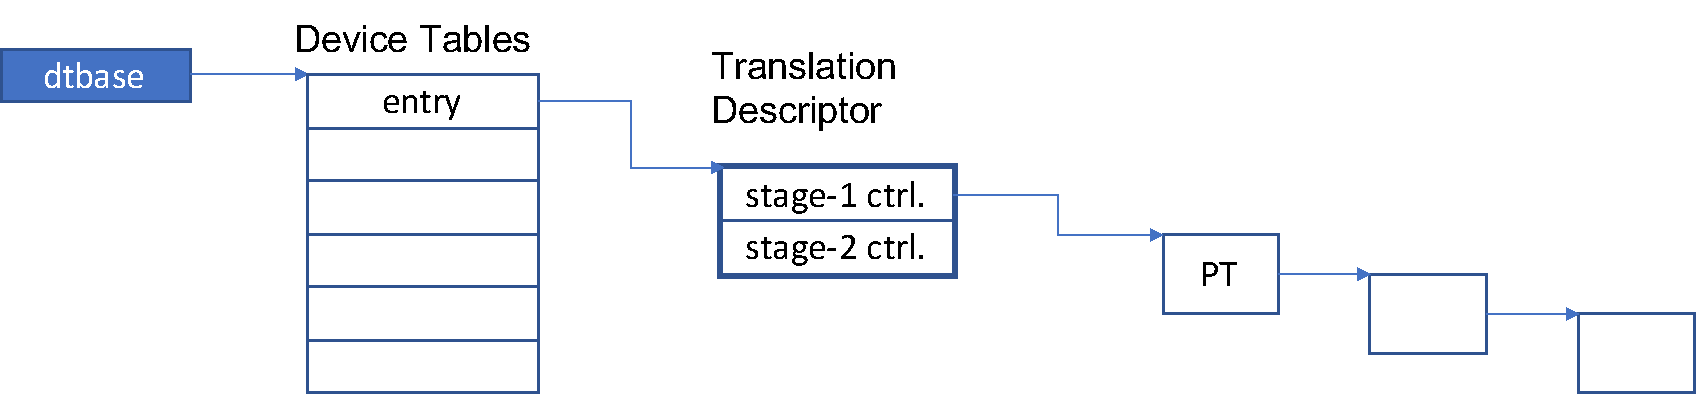
\includegraphics[width=0.95\textwidth]{img/one-stage-trans.pdf}
    \caption{One-Stage Translation}
    \label{fig:one-stage-trans}
\end{figure}

The translation table walk is in principle the same as the page table walk of the MMU,
however, the IOMMU uses the bits in the entries differently. Section \ref{sec:addr_tbl}
lists the bits that are used by the IOMMU.

\subsubsection{Translation with the Second Stage}

When S2MODE is not zero, stage-two translation is enabled. The RPAddr (Register Page
Address) field in the Stage One Control field contains the PPN of the memory space, called
register MMIO page, allocated by the system software, e.g a hypervisor, as the register
MMIO range for the virtual machine. The bytes inside the register MMIO page at the offset
of \dtbase\ contains the guest PPN for the device table defined by the virtual machine,
with which the it may define further translation tables.

\note The system software may also choose to not expose an IOMMU to the virtual machine,
in which case the system software simply provide a dummy register MMIO page for the
virtual machine. All such virtual machines without an IOMMU can share this dummy page,
minimizing memory overhead. \noteend

If the virtual machine does not enable any address translation for the devices assigned to
it, the IOMMU performs translation with only the second stage. Otherwise, the IOMMU
performs both stages of translation, in which the first stage is nested.

The hypervisor is expected to emulate the register MMIO range which include the
\dtbase\ register. When a VM attempts to write to the emulated \dtbase\
register, the hypervisor allocates a physical memory page to hold the values. This
approach keeps the code consistent between the guest VM and the host. 

When the device tables are implemented as MMIO registers, the \dtbase\ register is not
defined. In this case, the memory used to emulate the register MMIO range contains the
device table registers.

The hypervisor is also expected to emulate the command MMIO range. On a write to the
\invltlb\ register, the hypervisor performs the necessary invalidation and
synchronization on the IOMMU TLB. The details of the IOMMU TLB is provided in Section
\ref{sec:tlb}.

\begin{figure}[ht!]
    \centering
    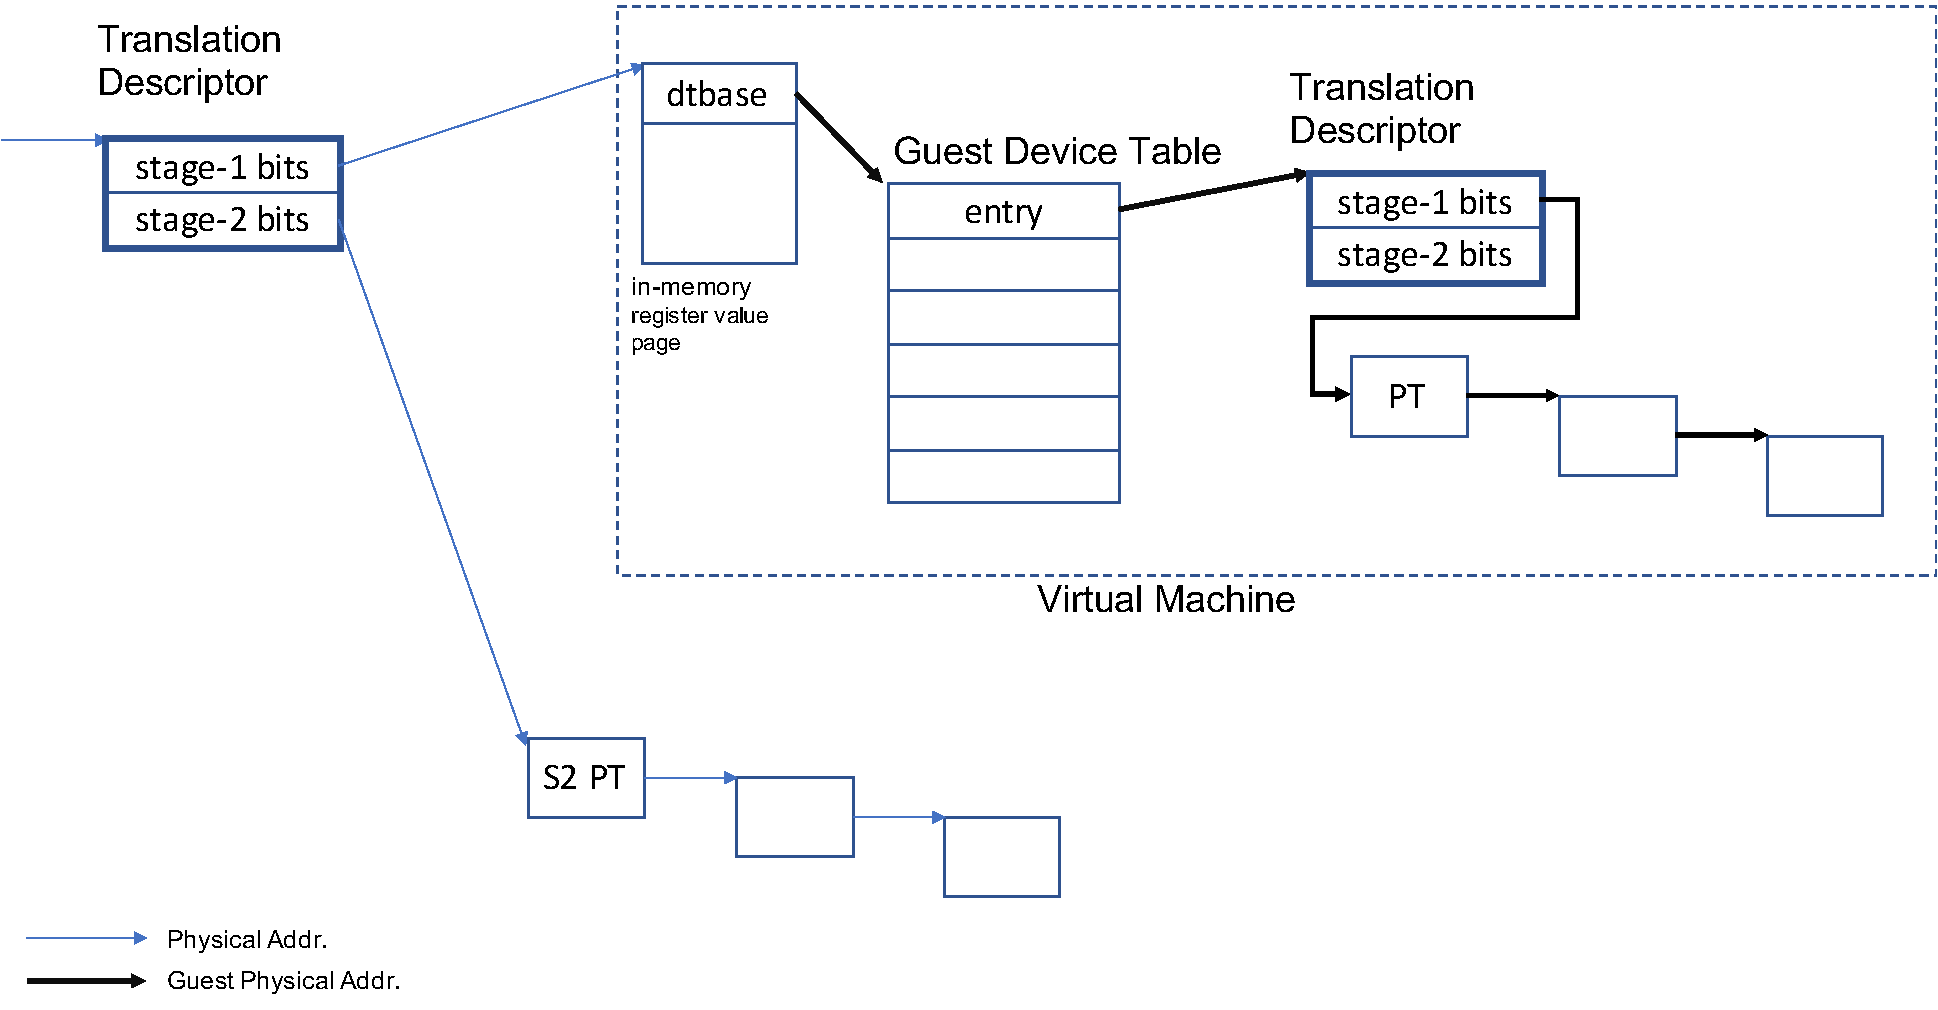
\includegraphics[width=0.95\textwidth]{img/two-stage-trans.pdf}
    \caption{Two-Stage Translation}
    \label{fig:two-stage-trans}
\end{figure}

On a translation request, the IOMMU obtains from the host device table the register page
base address, read the \textit{dtbase} value from the register page, then walks the
address tables pointed to by the guest device table. For each step in the table walk, the
GPAs are translated by the stage-two translation tables pointed to by the host device
table entry. At the end of the table walk, the IOMMU produces a physical address for the
translation request. Figure \ref{fig:two-stage-trans} illustrate the process. Note that
the device table look ups are simplified. 

If there's any fault detected during the table walk, the IOMMU may report the fault as
described in Section \ref{sec:fault} depending on the nature of the fault and the
configuration of the device.


\subsubsection{Update Notification}

Whenever the software updates any the address tables, the register \invltlb\ should be
written to with the RSID of the device whose translation is modified, so that the IOMMU
can perform necessary updates of the internal state. The \invltlb\ register resides in the
command MMIO range. The format of the \invltlb\ register is shown in Figure
\ref{fig:invltlb_reg}.

When the device tables are memory-resident, \invltlb\ is also used to invalid any cached
content inside the IOMMU. However, if the device tables are implemented as MMIO registers,
writing to \invltlb\ is not needed.

A write to the \invltlb\ register is mandatory for the initial setup of the device table.


\begin{figure}[ht!]

    \begin{center}
        \begin{tabular}{@{}T@{}K}
        \instbitrange{63}{\rsidlen} &
        \instbitrange{\rsidlen - 1}{0} \\
        \hline
        \multicolumn{1}{|c|}{Reserved} &
        \multicolumn{1}{ c|}{RSID} \\
        \hline
        63 - \rsidlen & \rsidlen \\
        \end{tabular}
    \end{center}

    \caption{The Format of the \invltlb\ Register}
    \label{fig:invltlb_reg}
\end{figure}


